\subsection{\en{Support Vector Machines}}
\en{Support Vector Machines are a family of models that are used for classification and regression analysis. The model was initially introduced by C. Cortes and V. Vapnik and has enjoyed considerable popularity since its creation, being one of the most widely used Machine Learning Techniques. They have been applied to many scientific fields, such as pattern recognition, image classification, biomedical research, petroleum exploration, etc.(\cite{57}, \cite{58}, \cite{59})  

The goal of an SVM is to choose a hyperplane (e.g. a straight line in two-dimensional space, a plane in three-dimensional) that best separates a dataset consisting of labeled samples that belong to one of two classes. The method that SVMs rely on to achieve this goal is choosing two parallel hyperplanes that separate the two classes such that the distance between them (the margin) is maximal. The data points on the margin maximizing hyperplanes (supporting vectors)  define the decision surface for the classification, as shown below: \cite{60}

\bigbreak
\begin{figure}[h!]
    \centering
    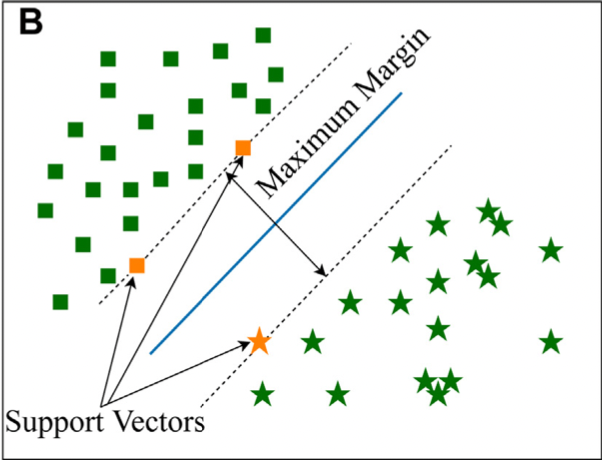
\includegraphics[width=0.5\textwidth]{figures/Theoretical_Background/SVM.png}
    \caption{\en{Support Vectors are shown in orange, the decision boundary in blue, the datapoints in green (squares for one class, stars for the other), and the dash lines are the margin maximizing hyperplanes. \cite{60}}}
\end{figure}
\bigbreak

SVMs can be used for multi-class classification as well, through a one-vs-one scheme or one-vs-rest approach, where decision boundaries are calculated between respective classes or a class and the rest of the dataset in each case, respectively. \cite{61}

SVMs enjoy a variety of advantages, such as efficiency in both low and high dimensional spaces, memory efficiency, and being able to produce results in cases where the number of samples is less than the number of dimensions. \cite{62}

However, one major drawback of SVMs is that the standard model does not work on datasets that are not linearly separable; that is one hyperplane cannot correctly divide the classes. To get around that, SVMs use kernels. Thus, the dataset is first non-linearly mapped through a kernel in a higher dimension space where the data is linearly separable, and then the original SVM algorithm is performed. In this approach, one can use the kernel trick to compute the transformations through the kernel function for the whole dataset. \cite{60}

SMVs suffer from over-fitting issues, as well as being sensitive to parameter selection/tuning, such as the kernel function and regularization term choice, especially if the number of parameters is much greater than the number of available samples. Additionally, SVMs are not scale invariant, so scaling the dataset is highly recommended. (\cite{62}, \cite{63}
}